\graphicspath{{./Lecture5/}}

\section{Bessel's Equation, continued from last class}

$$a_0 (r(r-1) + r - \nu^2) x^r + a_1 \left((1+r)r + (1+r) - \nu^2 \right) x^{r+1} + \sum_{n = 2}^\infty a_n \left(... \right) x^{n+r} = 0$$

We can use linear independency. This means that the set of the coefficients of all powers of $x$ must be zero.

The following is found from the characteristic equation:

$$x^r | a_0 (r^2 - \nu^2) = 0 \longrightarrow r = \pm \nu \text{ }\& \text{ } a_0 \neq 0$$

$$x^{r+1} | a_1 \left(r^2 + 2r + 1 - \nu^2 \right) = 0 \underbrace{\longrightarrow}_{\nu^2 - r^2} a_1 (2 \nu + 1) = 0$$

$$\hookrightarrow \left\{ \begin{matrix} \nu = \pm \frac{1}{2} &  \& & q \neq 0 \\ \nu \neq \pm \frac{1}{2} & \& & q = 0 \end{matrix} \right.$$

$$x^{n+r} | \left((n+r) (n+r-1) + (n+r) - \nu^2 \right) a_n + a_{n-2} = 0 \longrightarrow n \geq 2$$

$$(**)\text{ } a_n = \frac{-a_{n-2}}{(n+r)^2 - \nu^2}$$

Find the recursive relation for $r = \pm \nu$:

$r_1 = \nu$: $a_n = \frac{-a_{n-2}}{(n+\nu)^2 - \nu^2} = \frac{-a_{n-2}}{n(n + 2 \nu)}$,  $(n \geq 2)$

*writing down $a_2$, $a_3$, and $a_4$*

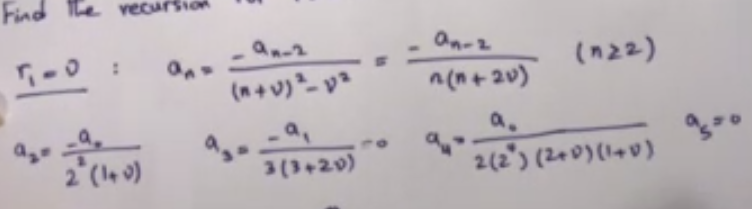
\includegraphics[width = 0.8 \textwidth]{image2.png}

\hfill

$\Rightarrow a_{2m} = \frac{(-)^m a_0}{m! 2^{2m} (1 + \nu) (2 + \nu) ... (m + \nu)}$

$$y_1(x) = a_0 x^{\nu} \sum_{m = 0}^\infty \frac{(-1)^m x^{2m}}{m! 2^{2m} (1 + \nu)(2 + \nu) ... (m + \nu)}$$

Now, for $r_1 = \nu$:

$$a_n = \frac{-1_{n-1}}{(n - \nu)^2 - \nu^2} = -\frac{a_{n-2}}{n(n - 2 \nu)}; n \geq 2$$

$$a_2 = \frac{-a_0}{2(2-2\nu)} = \frac{-a_0}{2(2)(1-\nu)}$$

$$a_4 = \frac{-a_2}{4(4-2\nu)} = \frac{a_0}{4(2)(2-\nu)(2^2)(1 - \nu)}$$

$$a_6 = \frac{-a_4}{6(6 - 2 \nu)} = \frac{-a_0}{6(2)(3-\nu)2^5 (2 - \nu) (1 - \nu)}$$

Note that $a_1 = a_3 = a_5 .... = 0$

$$\Rightarrow a_{2m} = \frac{(-1)^m a_0}{m! 2^{2m} (1-\nu)(2 - \nu) (3 - \nu) ... (m - \nu)}$$

$$ y_2(x) = a_0 x^{-\nu} \sum_{m = 0}^\infty \frac{(-1)^m a_0}{m! 2^{2m} (1-\nu)(2 - \nu) ... (m - \nu)}$$

Finally, $y(x)$ is a linear combination of 2 solutions:

$$y(x) = C_1 x^{\nu} \underbrace{\sum_{m = 0}^\infty \frac{(-1)^m (x/2)^{2m}}{m (1 + \nu)(2 + \nu) ... (m + \nu)}}_{J_\nu \text{: Bessel Functions of the first kind}} + C_2 \underbrace{x^{-\nu} \sum_{m = 0}^\infty \frac{(-1)^m a_0}{m! 2^{2m} (1-\nu)(2 - \nu) ... (m - \nu)}}_{Y_\nu \text{: Bessel function of the second kind}}$$

We will be given this in the formula sheet. Note that $C_1$ and $C_2$ are not included in $J_\nu$ and $Y_\nu$.

For $\nu \neq \pm \frac{1}{2}$: As $x \to  0$, $J_\nu \to 0$ and $x \to  0$, $Y_\nu \to \infty$

What happens when $\nu = 0$?

$$x^r | a_0 (r^2 - \nu^2) = 0 \rightarrow r = \pm \nu, a_0 \neq 0$$

Two solutions are the same. Therefore, $r_{1,2} = 0$


Then, $J_\nu(x) = C_1 x^0 \sum_{m = 0}^\infty \frac{(-1)^m}{(m!)^2} \left(\frac{x}{2} \right)^{2m}$

How about $Y_\nu (x)$?

Similar to Euler's equation (Refer to section 5.4 of the textbook), the second solution for repeated roots is:

$$y_2 (x) = y_1(x) \ln(x) + x^{r_1} \sum_{n = 1}^\infty a_n ' (r_1) x^n$$

where $a_n ' (r_1) = \left. \frac{d a_1}{dr} \right|_{r = r_1}$

According to this formula, $y_0 = J_0 (x) \ln(x) + x^{0} \sum_{n = 1}^\infty a_n' (0) x^n$ (***)

The recursion for this case (**) is found to be 

$$a_{2m} (r) = - \frac{a_{2m-2}}{(r + 2m)^2}, m = 1,2,3,...$$

$$a_{2m}(r) = \frac{(-1)^m a_0}{(r+2)^2 .... (r + 2m)^2}$$

$$a_{2m}' (r) = -2 \left( \frac{1}{r+2} + \frac{1}{r+4} + ... + \frac{1}{r + 2m} \right) a_{2m} (r)$$

$$a_{2m}' (0) = -2 \left( \frac{1}{2} + \frac{1}{4} + .... + \frac{1}{2m} \right) a_{2m}(0) = - \left(\frac{1}{2} + \frac{1}{4} + .... + \frac{1}{2m} \right) \frac{(-1)^m a_0}{2^{2m} (m!)^2} $$

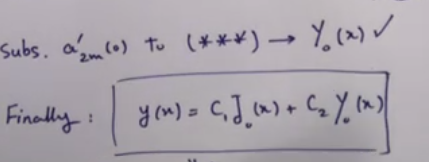
\includegraphics[width = 0.8 \textwidth]{image3.png}

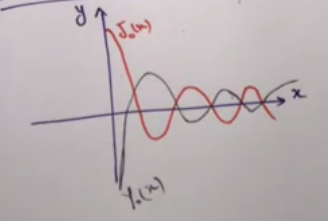
\includegraphics[width = 0.8 \textwidth]{image4.png}

As $x \to 0$, $y_0 (x) \to - \infty$, i.e. if the solution, $y(x)$, is finite at zero, then $C_2 = 0$

\section{Bessel Equation of Order of $\pm \frac{1}{2}$}

$$Ly = x^2 y'' + xy' + (x^2 - \frac{1}{4} )y = 0$$

$$x^r | a_0 (r^2 - \nu^2) = 0 \longrightarrow a_0 \neq 0 \text{ and } r = \pm \nu$$

For $\nu = \frac{1}{2} \Rightarrow r = \pm \frac{1}{2}$

$$x^{r+1} | a_1 (r^2 + 2r + 1 - \nu^2) = 0 \Rightarrow a_1 (1 \pm 2 \nu) = 0$$

If $\nu = \pm \frac{1}{2}$, $a_1$ is arbitrary

$$x^{m+r} | -a_m (r^2 + 2r + 1 - \nu^2) = a_{m=2} \Rightarrow a_m = \frac{-a_{m-2}}{(m+r)^2 - \nu^2}$$

For $\nu \pm \frac{1}{2}, a_m = \frac{-a_{m-2}}{(m+\frac{1}{2})^2 - \frac{1}{4}} = \frac{-a_{m-2}}{m(m+1)}$

Let $r_1 = \frac{1}{2}$: $a_1 (1 + 2 (\frac{1}{2})) = 0 \Rightarrow a_1 = 0$

$a_2 = - \frac{a_0}{2(3)}$, $a_4 = \frac{-a_2}{3(4)} = \frac{a_0}{5!}$

Therefore:

$$y_1 (x) = a_0 x^{\frac{1}{2}} \underbrace{\left(1 - \frac{x^2}{3!} + \frac{x^4}{5!} + ... \right) \frac{x}{x}}_{\text{Taylor series for } \sin(x)}$$

$$y_1(x) = a_0 x^{- \frac{1}{2}} \sin(x)$$

let $r_2 = \frac{-1}{2}$: $a_1 (1 - 2 \frac{1}{2}) = 0 \Rightarrow$ $a_1$ is arbitrary. it could be another solution.


for this case, $a_m = \frac{-a_{m - 2}}{(m = \frac{1}{2})^2 - \frac{1}{4}} = \frac{-a_{m - 2}}{m(m-1)}$

$a_2 = \frac{-a_0}{2(1)}$, $a_4 = \frac{-a_2}{4(3)} = \frac{a_0}{4!}$

$$\Rightarrow y_x(x) = a_0 x^{\frac{-1}{2}} \left(1 - \frac{x^2}{2!} + \frac{x^4}{4!} - ... \right) = a_0 x^{- \frac{1}{2}} \cos(x)$$

Let's check for $a_1 \neq 0$:

$a_3 = \frac{-a_1}{3 \cdot 2}$, $a_5 = \frac{-a_3}{5 \cdot 4} = \frac{a_1}{5!}$

$y_3 (x) = a_1 x^{- \frac{1}{2}} \sin(x)$. But this doesn't give us another solution -- This is the same as $y_1$; they are not independent. 

Hence we write the final solution as:

$$y(x) = a_0 x^{\frac{-1}{2}} \cos(x) + a_1 x^{\frac{-1}{2}} \sin(x)$$

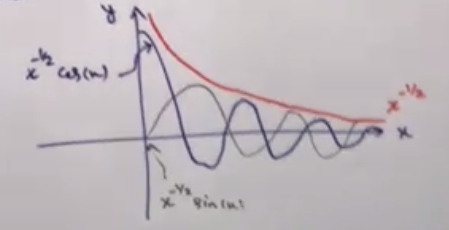
\includegraphics[width = 0.9 \textwidth]{image5.png}

\textbf{End of series functions}

\section{Introduction to PDE Classification}

What is a PDE?

A differential equation that includes partial derivatives with respect to all independent variables. 

$u(x,t) \longrightarrow$ PDEs include $\frac{\partial u}{\partial t}$, $\frac{\partial u}{\partial x}$, $\frac{\partial^2 u}{\partial x \partial t}$, $\frac{\partial^2 u}{\partial x^2}$, ...

\begin{itemize}
    \item Heat equation
    \item Wave equation
    \item Laplace equation
\end{itemize}